\documentclass{article}

\usepackage{arxiv}

\usepackage[utf8]{inputenc} % allow utf-8 input
\usepackage[T1]{fontenc}    % use 8-bit T1 fonts
\usepackage{lmodern}        % https://github.com/rstudio/rticles/issues/343
\usepackage{hyperref}       % hyperlinks
\usepackage{url}            % simple URL typesetting
\usepackage{booktabs}       % professional-quality tables
\usepackage{amsfonts}       % blackboard math symbols
\usepackage{nicefrac}       % compact symbols for 1/2, etc.
\usepackage{microtype}      % microtypography
\usepackage{lipsum}
\usepackage{graphicx}

\title{Longitudinal Data Cleaning - A Case of the NLSY79 Data}

\author{
    Dewi Amaliah
    \thanks{Use footnote for providing further information about author (webpage,
alternative address)---\emph{not} for acknowledging funding agencies.
Optional.}
   \\
    Department of Econometric and Business Statistics \\
    Monash University \\
  Clayton, VIC 3168 \\
  \texttt{\href{mailto:dama0007@student.monash.edu}{\nolinkurl{dama0007@student.monash.edu}}} \\
   \And
    Dianne Cook
   \\
    Department of Econometric and Business Statistics \\
    Monash University \\
  Clayton, VIC 3168 \\
  \texttt{\href{mailto:dicook@monash.edu}{\nolinkurl{dicook@monash.edu}}} \\
  }

\usepackage{color}
\usepackage{fancyvrb}
\newcommand{\VerbBar}{|}
\newcommand{\VERB}{\Verb[commandchars=\\\{\}]}
\DefineVerbatimEnvironment{Highlighting}{Verbatim}{commandchars=\\\{\}}
% Add ',fontsize=\small' for more characters per line
\usepackage{framed}
\definecolor{shadecolor}{RGB}{248,248,248}
\newenvironment{Shaded}{\begin{snugshade}}{\end{snugshade}}
\newcommand{\AlertTok}[1]{\textcolor[rgb]{0.94,0.16,0.16}{#1}}
\newcommand{\AnnotationTok}[1]{\textcolor[rgb]{0.56,0.35,0.01}{\textbf{\textit{#1}}}}
\newcommand{\AttributeTok}[1]{\textcolor[rgb]{0.77,0.63,0.00}{#1}}
\newcommand{\BaseNTok}[1]{\textcolor[rgb]{0.00,0.00,0.81}{#1}}
\newcommand{\BuiltInTok}[1]{#1}
\newcommand{\CharTok}[1]{\textcolor[rgb]{0.31,0.60,0.02}{#1}}
\newcommand{\CommentTok}[1]{\textcolor[rgb]{0.56,0.35,0.01}{\textit{#1}}}
\newcommand{\CommentVarTok}[1]{\textcolor[rgb]{0.56,0.35,0.01}{\textbf{\textit{#1}}}}
\newcommand{\ConstantTok}[1]{\textcolor[rgb]{0.00,0.00,0.00}{#1}}
\newcommand{\ControlFlowTok}[1]{\textcolor[rgb]{0.13,0.29,0.53}{\textbf{#1}}}
\newcommand{\DataTypeTok}[1]{\textcolor[rgb]{0.13,0.29,0.53}{#1}}
\newcommand{\DecValTok}[1]{\textcolor[rgb]{0.00,0.00,0.81}{#1}}
\newcommand{\DocumentationTok}[1]{\textcolor[rgb]{0.56,0.35,0.01}{\textbf{\textit{#1}}}}
\newcommand{\ErrorTok}[1]{\textcolor[rgb]{0.64,0.00,0.00}{\textbf{#1}}}
\newcommand{\ExtensionTok}[1]{#1}
\newcommand{\FloatTok}[1]{\textcolor[rgb]{0.00,0.00,0.81}{#1}}
\newcommand{\FunctionTok}[1]{\textcolor[rgb]{0.00,0.00,0.00}{#1}}
\newcommand{\ImportTok}[1]{#1}
\newcommand{\InformationTok}[1]{\textcolor[rgb]{0.56,0.35,0.01}{\textbf{\textit{#1}}}}
\newcommand{\KeywordTok}[1]{\textcolor[rgb]{0.13,0.29,0.53}{\textbf{#1}}}
\newcommand{\NormalTok}[1]{#1}
\newcommand{\OperatorTok}[1]{\textcolor[rgb]{0.81,0.36,0.00}{\textbf{#1}}}
\newcommand{\OtherTok}[1]{\textcolor[rgb]{0.56,0.35,0.01}{#1}}
\newcommand{\PreprocessorTok}[1]{\textcolor[rgb]{0.56,0.35,0.01}{\textit{#1}}}
\newcommand{\RegionMarkerTok}[1]{#1}
\newcommand{\SpecialCharTok}[1]{\textcolor[rgb]{0.00,0.00,0.00}{#1}}
\newcommand{\SpecialStringTok}[1]{\textcolor[rgb]{0.31,0.60,0.02}{#1}}
\newcommand{\StringTok}[1]{\textcolor[rgb]{0.31,0.60,0.02}{#1}}
\newcommand{\VariableTok}[1]{\textcolor[rgb]{0.00,0.00,0.00}{#1}}
\newcommand{\VerbatimStringTok}[1]{\textcolor[rgb]{0.31,0.60,0.02}{#1}}
\newcommand{\WarningTok}[1]{\textcolor[rgb]{0.56,0.35,0.01}{\textbf{\textit{#1}}}}

% Pandoc citation processing

\usepackage{booktabs}
\usepackage{longtable}
\usepackage{array}
\usepackage{multirow}
\usepackage{wrapfig}
\usepackage{float}
\usepackage{colortbl}
\usepackage{pdflscape}
\usepackage{tabu}
\usepackage{threeparttable}
\usepackage{threeparttablex}
\usepackage[normalem]{ulem}
\usepackage{makecell}
\usepackage{xcolor}


\begin{document}
\maketitle

\def\tightlist{}


\begin{abstract}
Enter the text of your abstract here.
\end{abstract}

\keywords{
    longitudinal data
   \and
    data cleaning
   \and
    data tidying
   \and
    robust linear model
  }

\hypertarget{introduction}{%
\section{Introduction}\label{introduction}}

\hypertarget{the-nlsy79}{%
\section{The NLSY79}\label{the-nlsy79}}

\hypertarget{the-nlsy79-data-cleaning}{%
\section{The NLSY79 Data Cleaning}\label{the-nlsy79-data-cleaning}}

\hypertarget{getting-and-tyding-the-data}{%
\subsection{Getting and Tyding the
Data}\label{getting-and-tyding-the-data}}

The NLYS data is stored in a
\href{https://www.nlsinfo.org/content/cohorts/nlsy79/get-data}{database}
and could be downloaded by variables. Several variables are available to
be downloaded and could be browsed by index. For the wages data set, we
only extracted these variables:

\begin{itemize}
\tightlist
\item
  Education, Training \& Achievement Scores

  \begin{itemize}
  \tightlist
  \item
    Education -\textgreater{} Summary measures -\textgreater{} All
    schools -\textgreater{} By year -\textgreater{} Highest grade
    completed

    \begin{itemize}
    \tightlist
    \item
      Downloaded all of the 78 variables in Highest grade completed.
    \end{itemize}
  \end{itemize}
\item
  Employment

  \begin{itemize}
  \tightlist
  \item
    Summary measures -\textgreater{} By job -\textgreater{} Hours worked
    and Hourly wages

    \begin{itemize}
    \tightlist
    \item
      Downloaded all of the 427 variables in Hours worked
    \item
      Downloaded all of the 151 variables in Hourly wages
    \end{itemize}

    Both hours worked and hourly wages are recorded by the job, up to
    five jobs for each id/subject.
  \end{itemize}
\item
  Household, Geography \& Contextual Variables

  \begin{itemize}
  \tightlist
  \item
    Context -\textgreater{} Summary measures -\textgreater{} Basic
    demographics

    \begin{itemize}
    \tightlist
    \item
      Downloaded year and month of birth, race, and sex variables.
    \end{itemize}

    There are two versions of the year and month of birth, i.e.~1979 and
    1981 data. We downloaded these two versions.
  \end{itemize}
\end{itemize}

The downloaded data set came in a csv (NLSY79.csv) and dat (NLSY79.dat)
format. We only used the .dat format. It also came along with these
files:

\begin{itemize}
\tightlist
\item
  NLSY79.NLSY79: This is the tagset of variables that can be uploaded to
  the web site to recreate the data set.
\item
  NLSY79.R: This is an R script provided automatically by the database
  for reading the data into R and convert the variables' name and its
  label into something more sensible. We utilized this code to do an
  initial data tidying. It produced two data set,
  \texttt{categories\_qnames} (the observations are stored in
  categorical/interval values) and \texttt{new\_data\_qnames} (the
  observations are stored in integer form). In this case, we only used
  the latter.
\end{itemize}

\begin{Shaded}
\begin{Highlighting}[]
\KeywordTok{source}\NormalTok{(here}\OperatorTok{::}\KeywordTok{here}\NormalTok{(}\StringTok{"data-raw/NLSY79/NLSY79.R"}\NormalTok{))}
\end{Highlighting}
\end{Shaded}

\texttt{new\_data\_qnames} is still untidy, where all of the variables
for each year and each job being stored in one column, hence the data
contains a huge number of columns (686 columns). Thus, the data should
be tidied and wrangled first to extract the demographic and employment
variables that we want to put in the final data set. We mainly used
\texttt{tidyr} (Wickham 2020), \texttt{dplyr} (Wickham et al. 2020), and
\texttt{stringr} (Wickham 2019) to do this job.

\hypertarget{tidying-demographic-variables}{%
\subsubsection{Tidying demographic
variables}\label{tidying-demographic-variables}}

\texttt{Age\ in\ 1979}, \texttt{gender}, \texttt{race},
\texttt{highest\ grade\ completed} (factor and integer), and the
\texttt{year\ when\ the\ highest\ grade\ completed} are the variables
that we want to use in the cleaned data set.

Age in 1979 are derived from year of birth and month of birth variables
in the raw data set. The variables have two versions, which are the 1979
version and the 1981 version. We only used the 1979 data and did a
consistency check of those years and flag the inconsistent observations.

\begin{Shaded}
\begin{Highlighting}[]
\CommentTok{## tidy the date of birth data}
\NormalTok{dob_tidy <-}\StringTok{ }\NormalTok{new_data_qnames }\OperatorTok
\StringTok{  }\NormalTok{dplyr}\OperatorTok{::}\KeywordTok{select}\NormalTok{(CASEID_}\DecValTok{1979}\NormalTok{,}
         \KeywordTok{starts_with}\NormalTok{(}\StringTok{"Q1-3_A~"}\NormalTok{)) }\OperatorTok
\StringTok{  }\KeywordTok{mutate}\NormalTok{(}\DataTypeTok{dob_year =} \KeywordTok{case_when}\NormalTok{(}
                    \CommentTok{# if the years recorded in both sets match, take 79 data}
                    \StringTok{`}\DataTypeTok{Q1-3_A~Y_1979}\StringTok{`} \OperatorTok{==}\StringTok{ `}\DataTypeTok{Q1-3_A~Y_1981}\StringTok{`} \OperatorTok{~}\StringTok{ `}\DataTypeTok{Q1-3_A~Y_1979}\StringTok{`}\NormalTok{,}
                    \CommentTok{# if the year in the 81 set is missing, take the 79 data}
                    \KeywordTok{is.na}\NormalTok{(}\StringTok{`}\DataTypeTok{Q1-3_A~Y_1981}\StringTok{`}\NormalTok{) }\OperatorTok{~}\StringTok{ `}\DataTypeTok{Q1-3_A~Y_1979}\StringTok{`}\NormalTok{,}
                    \CommentTok{# if the sets don't match for dob year, take the 79 data}
                    \StringTok{`}\DataTypeTok{Q1-3_A~Y_1979}\StringTok{`} \OperatorTok{!=}\StringTok{ `}\DataTypeTok{Q1-3_A~Y_1981}\StringTok{`} \OperatorTok{~}\StringTok{ `}\DataTypeTok{Q1-3_A~Y_1979}\StringTok{`}\NormalTok{),}
        \DataTypeTok{dob_month =} \KeywordTok{case_when}\NormalTok{(}
                    \CommentTok{# if months recorded in both sets match, take 79 data}
                    \StringTok{`}\DataTypeTok{Q1-3_A~M_1979}\StringTok{`} \OperatorTok{==}\StringTok{ `}\DataTypeTok{Q1-3_A~M_1981}\StringTok{`} \OperatorTok{~}\StringTok{ `}\DataTypeTok{Q1-3_A~M_1979}\StringTok{`}\NormalTok{,}
                    \CommentTok{# if month in 81 set is missing, take the 79 data}
                    \KeywordTok{is.na}\NormalTok{(}\StringTok{`}\DataTypeTok{Q1-3_A~M_1981}\StringTok{`}\NormalTok{) }\OperatorTok{~}\StringTok{ `}\DataTypeTok{Q1-3_A~M_1979}\StringTok{`}\NormalTok{,}
                    \CommentTok{# if sets don't match for dob month, take the 79 data}
                    \StringTok{`}\DataTypeTok{Q1-3_A~M_1979}\StringTok{`} \OperatorTok{!=}\StringTok{ `}\DataTypeTok{Q1-3_A~M_1981}\StringTok{`} \OperatorTok{~}\StringTok{ `}\DataTypeTok{Q1-3_A~M_1979}\StringTok{`}\NormalTok{),}
        \CommentTok{# flag if there is a conflict between dob recorded in 79 and 81}
        \DataTypeTok{dob_conflict =} \KeywordTok{case_when}\NormalTok{(     }
\NormalTok{                      (}\StringTok{`}\DataTypeTok{Q1-3_A~M_1979}\StringTok{`} \OperatorTok{!=}\StringTok{ `}\DataTypeTok{Q1-3_A~M_1981}\StringTok{`}\NormalTok{) }\OperatorTok{&}\StringTok{ }\OperatorTok{!}\KeywordTok{is.na}\NormalTok{(}\StringTok{`}\DataTypeTok{Q1-3_A~M_1981}\StringTok{`}\NormalTok{)}
                      \OperatorTok{~}\StringTok{ }\OtherTok{TRUE}\NormalTok{,}
\NormalTok{                      (}\StringTok{`}\DataTypeTok{Q1-3_A~Y_1979}\StringTok{`} \OperatorTok{!=}\StringTok{ `}\DataTypeTok{Q1-3_A~Y_1981}\StringTok{`}\NormalTok{) }\OperatorTok{&}\StringTok{ }\OperatorTok{!}\KeywordTok{is.na}\NormalTok{(}\StringTok{`}\DataTypeTok{Q1-3_A~Y_1981}\StringTok{`}\NormalTok{)}
                      \OperatorTok{~}\StringTok{ }\OtherTok{TRUE}\NormalTok{,}
\NormalTok{                      (}\StringTok{`}\DataTypeTok{Q1-3_A~Y_1979}\StringTok{`} \OperatorTok{==}\StringTok{ `}\DataTypeTok{Q1-3_A~Y_1981}\StringTok{`}\NormalTok{) }\OperatorTok{&}\StringTok{ }
\StringTok{                      }\NormalTok{(}\StringTok{`}\DataTypeTok{Q1-3_A~M_1979}\StringTok{`} \OperatorTok{==}\StringTok{ `}\DataTypeTok{Q1-3_A~M_1981}\StringTok{`}\NormalTok{) }\OperatorTok{~}\StringTok{ }\OtherTok{FALSE}\NormalTok{,}
                      \KeywordTok{is.na}\NormalTok{(}\StringTok{`}\DataTypeTok{Q1-3_A~M_1981}\StringTok{`}\NormalTok{) }\OperatorTok{|}\StringTok{ }\KeywordTok{is.na}\NormalTok{(}\StringTok{`}\DataTypeTok{Q1-3_A~Y_1981}\StringTok{`}\NormalTok{) }\OperatorTok{~}\StringTok{ }\OtherTok{FALSE}\NormalTok{)) }\OperatorTok
\StringTok{  }\NormalTok{dplyr}\OperatorTok{::}\KeywordTok{select}\NormalTok{(CASEID_}\DecValTok{1979}\NormalTok{,}
\NormalTok{         dob_month,}
\NormalTok{         dob_year,}
\NormalTok{         dob_conflict)}
\end{Highlighting}
\end{Shaded}

For \texttt{gender} and \texttt{race}, we only renamed these variables.

\begin{Shaded}
\begin{Highlighting}[]
\CommentTok{## tidy the gender and race variables}
\NormalTok{demog_tidy <-}\StringTok{ }\NormalTok{categories_qnames }\OperatorTok
\StringTok{  }\NormalTok{dplyr}\OperatorTok{::}\KeywordTok{select}\NormalTok{(CASEID_}\DecValTok{1979}\NormalTok{,}
\NormalTok{         SAMPLE_RACE_78SCRN,}
\NormalTok{         SAMPLE_SEX_}\DecValTok{1979}\NormalTok{) }\OperatorTok
\StringTok{  }\KeywordTok{rename}\NormalTok{(}\DataTypeTok{gender =}\NormalTok{ SAMPLE_SEX_}\DecValTok{1979}\NormalTok{,}
         \DataTypeTok{race =}\NormalTok{ SAMPLE_RACE_78SCRN)}
\end{Highlighting}
\end{Shaded}

The \texttt{highest\ grade\ completed} came with several version in each
year. We chose the revised May data because the May data seemed to have
less missing and presumably the revised data has been checked. However,
there was no revised May data for 2012, 2014, 2016, and 2018 so we just
used the ordinary May data.

\begin{Shaded}
\begin{Highlighting}[]
\CommentTok{# tidy the grade }
\NormalTok{demog_education <-}\StringTok{ }\NormalTok{new_data_qnames }\OperatorTok
\StringTok{  }\KeywordTok{as_tibble}\NormalTok{() }\OperatorTok
\StringTok{  }\CommentTok{# in 2018, the variable's name is Q3-4_2018, instead of HGC_2018}
\StringTok{  }\KeywordTok{rename}\NormalTok{(}\DataTypeTok{HGC_2018 =} \StringTok{`}\DataTypeTok{Q3-4_2018}\StringTok{`}\NormalTok{) }\OperatorTok
\StringTok{  }\NormalTok{dplyr}\OperatorTok{::}\KeywordTok{select}\NormalTok{(CASEID_}\DecValTok{1979}\NormalTok{,}
         \KeywordTok{starts_with}\NormalTok{(}\StringTok{"HGCREV"}\NormalTok{),}
         \StringTok{"HGC_2012"}\NormalTok{,}
         \StringTok{"HGC_2014"}\NormalTok{,}
         \StringTok{"HGC_2016"}\NormalTok{,}
         \StringTok{"HGC_2018"}\NormalTok{) }\OperatorTok
\StringTok{  }\KeywordTok{pivot_longer}\NormalTok{(}\OperatorTok{!}\NormalTok{CASEID_}\DecValTok{1979}\NormalTok{,}
               \DataTypeTok{names_to =} \StringTok{"var"}\NormalTok{,}
               \DataTypeTok{values_to =} \StringTok{"grade"}\NormalTok{) }\OperatorTok
\StringTok{  }\KeywordTok{separate}\NormalTok{(}\StringTok{"var"}\NormalTok{, }\KeywordTok{c}\NormalTok{(}\StringTok{"var"}\NormalTok{, }\StringTok{"year"}\NormalTok{), }\DataTypeTok{sep =} \DecValTok{-4}\NormalTok{) }\OperatorTok
\StringTok{  }\KeywordTok{filter}\NormalTok{(}\OperatorTok{!}\KeywordTok{is.na}\NormalTok{(grade)) }\OperatorTok
\StringTok{  }\NormalTok{dplyr}\OperatorTok{::}\KeywordTok{select}\NormalTok{(}\OperatorTok{-}\NormalTok{var)}
\end{Highlighting}
\end{Shaded}

In the final data, we only used the highest grade completed ever and
derived the year of when the highest grade completed its categorical
value. Therefore, we wrangled the highest grade completed in each year
to mutate these variables.

\begin{Shaded}
\begin{Highlighting}[]
\CommentTok{## getting the highest year of completed education ever}
\NormalTok{highest_year <-}\StringTok{ }\NormalTok{demog_education }\OperatorTok
\StringTok{  }\KeywordTok{group_by}\NormalTok{(CASEID_}\DecValTok{1979}\NormalTok{) }\OperatorTok
\StringTok{  }\KeywordTok{mutate}\NormalTok{(}\DataTypeTok{hgc_i =} \KeywordTok{max}\NormalTok{(grade)) }\OperatorTok
\StringTok{  }\KeywordTok{filter}\NormalTok{(hgc_i }\OperatorTok{==}\StringTok{ }\NormalTok{grade) }\OperatorTok
\StringTok{  }\KeywordTok{filter}\NormalTok{(year }\OperatorTok{==}\StringTok{ }\KeywordTok{first}\NormalTok{(year)) }\OperatorTok
\StringTok{  }\KeywordTok{rename}\NormalTok{(}\DataTypeTok{yr_hgc =}\NormalTok{ year) }\OperatorTok
\StringTok{  }\NormalTok{dplyr}\OperatorTok{::}\KeywordTok{select}\NormalTok{(CASEID_}\DecValTok{1979}\NormalTok{, yr_hgc, hgc_i) }\OperatorTok
\StringTok{  }\KeywordTok{ungroup}\NormalTok{() }\OperatorTok
\StringTok{  }\KeywordTok{mutate}\NormalTok{(}\StringTok{'hgc'}\NormalTok{ =}\StringTok{ }\KeywordTok{ifelse}\NormalTok{(hgc_i }\OperatorTok{==}\StringTok{ }\DecValTok{0}\NormalTok{, }\StringTok{"NONE"}\NormalTok{, }\KeywordTok{ifelse}\NormalTok{(hgc_i }\OperatorTok{==}\StringTok{ }\DecValTok{1}\NormalTok{, }\StringTok{"1ST GRADE"}\NormalTok{,}
                 \KeywordTok{ifelse}\NormalTok{(hgc_i }\OperatorTok{==}\StringTok{ }\DecValTok{2}\NormalTok{, }\StringTok{"2ND GRADE"}\NormalTok{, }\KeywordTok{ifelse}\NormalTok{(hgc_i }\OperatorTok{==}\StringTok{ }\DecValTok{3}\NormalTok{, }\StringTok{"3RD GRADE"}\NormalTok{,}
                 \KeywordTok{ifelse}\NormalTok{(hgc_i }\OperatorTok{>=}\StringTok{ }\DecValTok{4} \OperatorTok{&}\StringTok{ }\NormalTok{hgc_i }\OperatorTok{<=}\StringTok{ }\DecValTok{12}\NormalTok{, }\KeywordTok{paste0}\NormalTok{(hgc_i,}\StringTok{"TH GRADE"}\NormalTok{),}
                 \KeywordTok{ifelse}\NormalTok{(hgc_i }\OperatorTok{==}\StringTok{ }\DecValTok{13}\NormalTok{, }\StringTok{"1ST YEAR COL"}\NormalTok{,}
                 \KeywordTok{ifelse}\NormalTok{(hgc_i }\OperatorTok{==}\StringTok{ }\DecValTok{14}\NormalTok{, }\StringTok{"2ND YEAR COL"}\NormalTok{,}
                 \KeywordTok{ifelse}\NormalTok{(hgc_i }\OperatorTok{==}\StringTok{ }\DecValTok{15}\NormalTok{, }\StringTok{"3RD YEAR COL"}\NormalTok{,}
                 \KeywordTok{ifelse}\NormalTok{(hgc_i }\OperatorTok{==}\StringTok{ }\DecValTok{95}\NormalTok{, }\StringTok{"UNGRADED"}\NormalTok{, }
                        \KeywordTok{paste0}\NormalTok{((hgc_i }\OperatorTok{-}\StringTok{ }\DecValTok{12}\NormalTok{), }\StringTok{"TH YEAR COL"}\NormalTok{)))))))))))}
\end{Highlighting}
\end{Shaded}

Finally, we join all the tidy variables in a data set called
\texttt{full\_demographics}.

\begin{Shaded}
\begin{Highlighting}[]
\NormalTok{full_demographics <-}\StringTok{ }\KeywordTok{full_join}\NormalTok{(dob_tidy, demog_tidy, }\DataTypeTok{by =} \StringTok{"CASEID_1979"}\NormalTok{) }\OperatorTok
\StringTok{  }\KeywordTok{full_join}\NormalTok{(highest_year, }\DataTypeTok{by =} \StringTok{"CASEID_1979"}\NormalTok{) }\OperatorTok
\StringTok{  }\KeywordTok{rename}\NormalTok{(}\StringTok{"id"}\NormalTok{ =}\StringTok{ "CASEID_1979"}\NormalTok{)}

\KeywordTok{head}\NormalTok{(full_demographics)}
\end{Highlighting}
\end{Shaded}

\begin{verbatim}
##   id dob_month dob_year dob_conflict                    race gender yr_hgc
## 1  1         9       58        FALSE NON-BLACK, NON-HISPANIC FEMALE   1979
## 2  2         1       59        FALSE NON-BLACK, NON-HISPANIC FEMALE   1985
## 3  3         8       61        FALSE NON-BLACK, NON-HISPANIC FEMALE   1993
## 4  4         8       62        FALSE NON-BLACK, NON-HISPANIC FEMALE   1986
## 5  5         7       59        FALSE NON-BLACK, NON-HISPANIC   MALE   1984
## 6  6        10       60        FALSE NON-BLACK, NON-HISPANIC   MALE   1983
##   hgc_i          hgc
## 1    12   12TH GRADE
## 2    12   12TH GRADE
## 3    12   12TH GRADE
## 4    14 2ND YEAR COL
## 5    18 6TH YEAR COL
## 6    16 4TH YEAR COL
\end{verbatim}

\hypertarget{tidying-employment-variables}{%
\subsubsection{Tidying employment
variables}\label{tidying-employment-variables}}

The employment data comprises of three variables,
i.e.~\texttt{total\ hours\ of\ work\ per\ week},
\texttt{number\ of\ jobs\ that\ an\ individual\ has}, and
\texttt{mean\ hourly\ wage}. For hours worked per week, initially only
one version per job, no choice from 1979 to 1987 (QES-52A). From 1988
onward, when we had more options, we chose the variable for total hours
including time spent working from home (QES-52D). However, 1993 did not
have all the five D variables (the first one and the last one were
missing), so we used QES-52A variable instead. In addition, 2008 only
had jobs 1-4 for the QES-52D variable (whereas the other years had 1-5),
so we just used these.

\begin{Shaded}
\begin{Highlighting}[]
\CommentTok{# make a list for years where we used the "QES-52A"}
\NormalTok{year_A <-}\StringTok{ }\KeywordTok{c}\NormalTok{(}\DecValTok{1979}\OperatorTok{:}\DecValTok{1987}\NormalTok{, }\DecValTok{1993}\NormalTok{)}
\CommentTok{#function to get the hour of work}
\NormalTok{get_hour <-}\StringTok{ }\ControlFlowTok{function}\NormalTok{(year)\{}
  \ControlFlowTok{if}\NormalTok{(year }\OperatorTok\StringTok{ }\NormalTok{year_A)\{}
\NormalTok{   temp <-}\StringTok{ }\NormalTok{new_data_qnames }\OperatorTok
\StringTok{    }\NormalTok{dplyr}\OperatorTok{::}\KeywordTok{select}\NormalTok{(CASEID_}\DecValTok{1979}\NormalTok{,}
            \KeywordTok{starts_with}\NormalTok{(}\StringTok{"QES-52A"}\NormalTok{) }\OperatorTok{&}
\StringTok{              }\KeywordTok{ends_with}\NormalTok{(}\KeywordTok{as.character}\NormalTok{(year)))\} }
  \ControlFlowTok{else}\NormalTok{\{}
\NormalTok{    temp <-}\StringTok{ }\NormalTok{new_data_qnames }\OperatorTok
\StringTok{    }\NormalTok{dplyr}\OperatorTok{::}\KeywordTok{select}\NormalTok{(CASEID_}\DecValTok{1979}\NormalTok{,}
            \KeywordTok{starts_with}\NormalTok{(}\StringTok{"QES-52D"}\NormalTok{) }\OperatorTok{&}
\StringTok{              }\KeywordTok{ends_with}\NormalTok{(}\KeywordTok{as.character}\NormalTok{(year)))\} }
\NormalTok{    temp }\OperatorTok\StringTok{ }
\StringTok{      }\KeywordTok{pivot_longer}\NormalTok{(}\OperatorTok{!}\NormalTok{CASEID_}\DecValTok{1979}\NormalTok{,}
                 \DataTypeTok{names_to =} \StringTok{"job"}\NormalTok{,}
                 \DataTypeTok{values_to =} \StringTok{"hours_work"}\NormalTok{) }\OperatorTok
\StringTok{      }\KeywordTok{separate}\NormalTok{(}\StringTok{"job"}\NormalTok{, }\KeywordTok{c}\NormalTok{(}\StringTok{"job"}\NormalTok{, }\StringTok{"year"}\NormalTok{), }\DataTypeTok{sep =} \DecValTok{-4}\NormalTok{) }\OperatorTok
\StringTok{      }\KeywordTok{mutate}\NormalTok{(}\DataTypeTok{job =} \KeywordTok{paste0}\NormalTok{(}\StringTok{"job_"}\NormalTok{, }\KeywordTok{substr}\NormalTok{(job, }\DecValTok{9}\NormalTok{, }\DecValTok{10}\NormalTok{))) }\OperatorTok
\StringTok{      }\KeywordTok{rename}\NormalTok{(}\DataTypeTok{id =}\NormalTok{ CASEID_}\DecValTok{1979}\NormalTok{)}
\NormalTok{\}}

\CommentTok{# list to save the iteration result}
\NormalTok{hours <-}\StringTok{ }\KeywordTok{list}\NormalTok{()}
\CommentTok{# getting the hours of work of all observations}
\ControlFlowTok{for}\NormalTok{(ayear }\ControlFlowTok{in} \KeywordTok{c}\NormalTok{(}\DecValTok{1979}\OperatorTok{:}\DecValTok{1994}\NormalTok{, }\DecValTok{1996}\NormalTok{, }\DecValTok{1998}\NormalTok{, }\DecValTok{2000}\NormalTok{, }\DecValTok{2002}\NormalTok{, }\DecValTok{2004}\NormalTok{, }\DecValTok{2006}\NormalTok{, }\DecValTok{2008}\NormalTok{, }\DecValTok{2010}\NormalTok{, }
               \DecValTok{2012}\NormalTok{, }\DecValTok{2014}\NormalTok{, }\DecValTok{2016}\NormalTok{, }\DecValTok{2018}\NormalTok{)) \{}
\NormalTok{   hours[[ayear]] <-}\StringTok{ }\KeywordTok{get_hour}\NormalTok{(ayear)}
\NormalTok{\}}
\CommentTok{# unlist the hours of work}
\NormalTok{hours_all <-}\StringTok{ }\KeywordTok{bind_rows}\NormalTok{(}\OperatorTok{!!!}\NormalTok{hours)}
\end{Highlighting}
\end{Shaded}

The same algorithm was also deployed to tidy the rate of wage by year
and by ID. The difference is that the hourly rate had only one version
of each year. The hours of work and the hourly rate were then joined to
calculate the number of jobs that an ID has and their mean hourly wage.
Some observations had 0 in their hourly rate, which is considered as
invalid value. Thus, their hourly rate set to be N.A.

\begin{Shaded}
\begin{Highlighting}[]
\NormalTok{get_rate <-}\StringTok{ }\ControlFlowTok{function}\NormalTok{(year) \{}
\NormalTok{  new_data_qnames }\OperatorTok
\StringTok{    }\NormalTok{dplyr}\OperatorTok{::}\KeywordTok{select}\NormalTok{(CASEID_}\DecValTok{1979}\NormalTok{,}
            \KeywordTok{starts_with}\NormalTok{(}\StringTok{"HRP"}\NormalTok{) }\OperatorTok{&}
\StringTok{              }\KeywordTok{ends_with}\NormalTok{(}\KeywordTok{as.character}\NormalTok{(year))) }\OperatorTok
\StringTok{    }\KeywordTok{pivot_longer}\NormalTok{(}\OperatorTok{!}\NormalTok{CASEID_}\DecValTok{1979}\NormalTok{, }\DataTypeTok{names_to =} \StringTok{"job"}\NormalTok{, }\DataTypeTok{values_to =} \StringTok{"rate_per_hour"}\NormalTok{) }\OperatorTok
\StringTok{    }\KeywordTok{separate}\NormalTok{(}\StringTok{"job"}\NormalTok{, }\KeywordTok{c}\NormalTok{(}\StringTok{"job"}\NormalTok{, }\StringTok{"year"}\NormalTok{), }\DataTypeTok{sep =} \DecValTok{-4}\NormalTok{) }\OperatorTok
\StringTok{    }\KeywordTok{mutate}\NormalTok{(}\DataTypeTok{job =} \KeywordTok{paste0}\NormalTok{(}\StringTok{"job_0"}\NormalTok{, }\KeywordTok{substr}\NormalTok{(job, }\DecValTok{4}\NormalTok{, }\DecValTok{4}\NormalTok{))) }\OperatorTok
\StringTok{    }\KeywordTok{rename}\NormalTok{(}\DataTypeTok{id =}\NormalTok{ CASEID_}\DecValTok{1979}\NormalTok{)}
\NormalTok{\}}
\NormalTok{rates <-}\StringTok{ }\KeywordTok{list}\NormalTok{()}
\ControlFlowTok{for}\NormalTok{(ayear }\ControlFlowTok{in} \KeywordTok{c}\NormalTok{(}\DecValTok{1979}\OperatorTok{:}\DecValTok{1994}\NormalTok{, }\DecValTok{1996}\NormalTok{, }\DecValTok{1998}\NormalTok{, }\DecValTok{2000}\NormalTok{, }\DecValTok{2002}\NormalTok{, }\DecValTok{2004}\NormalTok{, }\DecValTok{2006}\NormalTok{, }\DecValTok{2008}\NormalTok{, }\DecValTok{2010}\NormalTok{, }
               \DecValTok{2012}\NormalTok{, }\DecValTok{2014}\NormalTok{, }\DecValTok{2016}\NormalTok{, }\DecValTok{2018}\NormalTok{)) \{}
\NormalTok{   rates[[ayear]] <-}\StringTok{ }\KeywordTok{get_rate}\NormalTok{(ayear)}
\NormalTok{\}}
\NormalTok{rates_all <-}\StringTok{ }\KeywordTok{bind_rows}\NormalTok{(}\OperatorTok{!!!}\NormalTok{rates)}
\CommentTok{# join hours and rates variable}
\NormalTok{hours_wages <-}\StringTok{ }\KeywordTok{left_join}\NormalTok{(rates_all, }
\NormalTok{                         hours_all, }
                         \DataTypeTok{by =} \KeywordTok{c}\NormalTok{(}\StringTok{"id"}\NormalTok{, }\StringTok{"year"}\NormalTok{, }\StringTok{"job"}\NormalTok{)) }\OperatorTok
\StringTok{  }\CommentTok{# set the 0 value in rate_per_hour as NA }
\StringTok{  }\KeywordTok{mutate}\NormalTok{(}\DataTypeTok{rate_per_hour =} \KeywordTok{ifelse}\NormalTok{(rate_per_hour }\OperatorTok{==}\StringTok{ }\DecValTok{0}\NormalTok{, }\OtherTok{NA}\NormalTok{,}
\NormalTok{                                rate_per_hour))}
\KeywordTok{head}\NormalTok{(hours_wages)}
\end{Highlighting}
\end{Shaded}

\begin{verbatim}
## # A tibble: 6 x 5
##      id job    year  rate_per_hour hours_work
##   <int> <chr>  <chr>         <int>      <int>
## 1     1 job_01 1979            328         38
## 2     1 job_02 1979             NA         15
## 3     1 job_03 1979             NA         NA
## 4     1 job_04 1979             NA         NA
## 5     1 job_05 1979             NA         NA
## 6     2 job_01 1979            385         35
\end{verbatim}

Since our ultimate goal is to calculate the mean hourly wage, the number
of jobs is calculate based on the availability of the
\texttt{rate\_per\_hour} information. For example, the number of jobs of
ID 1, based on \texttt{hours\_work}, is two. However, since the
information of hourly rate of \texttt{job\_02} is not available, the
number of job is considered as 1.

Further, we calculated the mean hourly wage for each ID in each year
using a weighted mean with the hours of work as the weight. However,
there are a lot of missing value in \texttt{hours\_work} variable. In
that case, we only calculated the mean hourly wage based on
arithmetic/regular mean method. Hence, we created a new variable to flag
whether the mean hourly wage is a weighted or a regular mean.
Additionally, if an ID only had one job, we directly used their hourly
wages information and flagged it as an arithmetic mean.

\begin{Shaded}
\begin{Highlighting}[]
\CommentTok{# calculate number of jobs that a person has in one year}
\NormalTok{no_job <-}\StringTok{ }\NormalTok{hours_wages }\OperatorTok
\StringTok{  }\KeywordTok{filter}\NormalTok{(}\OperatorTok{!}\KeywordTok{is.na}\NormalTok{(rate_per_hour)) }\OperatorTok
\StringTok{  }\KeywordTok{group_by}\NormalTok{(id, year) }\OperatorTok
\StringTok{  }\KeywordTok{summarise}\NormalTok{(}\DataTypeTok{no_jobs =} \KeywordTok{length}\NormalTok{(rate_per_hour))}

\CommentTok{# filter the observations with available rate per hour}
\NormalTok{eligible_wages <-}\StringTok{ }\NormalTok{hours_wages }\OperatorTok
\StringTok{  }\KeywordTok{filter}\NormalTok{(}\OperatorTok{!}\KeywordTok{is.na}\NormalTok{(rate_per_hour)) }\OperatorTok
\StringTok{  }\KeywordTok{left_join}\NormalTok{(no_job, }\DataTypeTok{by =} \KeywordTok{c}\NormalTok{(}\StringTok{"id"}\NormalTok{, }\StringTok{"year"}\NormalTok{)) }

\CommentTok{# calculate the mean_hourly_wage}
\CommentTok{# flag1 = code 1 for weighted mean}
\CommentTok{# code 0 for arithmetic mean}
\NormalTok{mean_hourly_wage <-}\StringTok{ }
\StringTok{  }\NormalTok{eligible_wages }\OperatorTok
\StringTok{  }\KeywordTok{group_by}\NormalTok{(id, year) }\OperatorTok
\StringTok{  }\CommentTok{#calculate the weighted mean if the number of jobs > 1}
\StringTok{  }\KeywordTok{mutate}\NormalTok{(}\DataTypeTok{wages =} \KeywordTok{ifelse}\NormalTok{(no_jobs }\OperatorTok{==}\StringTok{ }\DecValTok{1}\NormalTok{, rate_per_hour}\OperatorTok{/}\DecValTok{100}\NormalTok{,}
                        \KeywordTok{weighted.mean}\NormalTok{(rate_per_hour, hours_work, }\DataTypeTok{na.rm =} \OtherTok{TRUE}\NormalTok{)}\OperatorTok{/}\DecValTok{100}\NormalTok{)) }\OperatorTok
\StringTok{  }\CommentTok{#give the flag if it the weighted mean}
\StringTok{  }\KeywordTok{mutate}\NormalTok{(}\DataTypeTok{flag1 =} \KeywordTok{ifelse}\NormalTok{(}\OperatorTok{!}\KeywordTok{is.na}\NormalTok{(wages) }\OperatorTok{&}\StringTok{ }\NormalTok{no_jobs }\OperatorTok{!=}\StringTok{ }\DecValTok{1}\NormalTok{, }\DecValTok{1}\NormalTok{,}
                        \DecValTok{0}\NormalTok{)) }\OperatorTok
\StringTok{  }\CommentTok{#calculate the arithmetic mean for the na}
\StringTok{  }\KeywordTok{mutate}\NormalTok{(}\DataTypeTok{wages =} \KeywordTok{ifelse}\NormalTok{(}\KeywordTok{is.na}\NormalTok{(wages), }\KeywordTok{mean}\NormalTok{(rate_per_hour)}\OperatorTok{/}\DecValTok{100}\NormalTok{,}
\NormalTok{                        wages)) }\OperatorTok
\StringTok{  }\KeywordTok{group_by}\NormalTok{(id, year) }\OperatorTok
\StringTok{  }\KeywordTok{summarise}\NormalTok{(}\DataTypeTok{wages =} \KeywordTok{mean}\NormalTok{(wages),}
            \DataTypeTok{total_hours =} \KeywordTok{sum}\NormalTok{(hours_work),}
            \DataTypeTok{number_of_jobs =} \KeywordTok{mean}\NormalTok{(no_jobs),}
            \DataTypeTok{flag1 =} \KeywordTok{mean}\NormalTok{(flag1)) }\OperatorTok
\StringTok{  }\KeywordTok{mutate}\NormalTok{(}\DataTypeTok{year =} \KeywordTok{as.numeric}\NormalTok{(year)) }\OperatorTok
\StringTok{  }\KeywordTok{ungroup}\NormalTok{() }\OperatorTok
\StringTok{  }\KeywordTok{rename}\NormalTok{(}\DataTypeTok{mean_hourly_wage =}\NormalTok{ wages) }\OperatorTok
\StringTok{  }\KeywordTok{mutate}\NormalTok{(}\DataTypeTok{is_wm =} \KeywordTok{ifelse}\NormalTok{(flag1 }\OperatorTok{==}\StringTok{ }\DecValTok{1}\NormalTok{, }\OtherTok{TRUE}\NormalTok{,}
                        \OtherTok{FALSE}\NormalTok{)) }\OperatorTok
\StringTok{  }\NormalTok{dplyr}\OperatorTok{::}\KeywordTok{select}\NormalTok{(}\OperatorTok{-}\NormalTok{flag1)}

\KeywordTok{head}\NormalTok{(mean_hourly_wage, }\DataTypeTok{n =} \DecValTok{10}\NormalTok{)}
\end{Highlighting}
\end{Shaded}

\begin{verbatim}
## # A tibble: 10 x 6
##       id  year mean_hourly_wage total_hours number_of_jobs is_wm
##    <int> <dbl>            <dbl>       <int>          <dbl> <lgl>
##  1     1  1979             3.28          38              1 FALSE
##  2     1  1981             3.61          NA              1 FALSE
##  3     2  1979             3.85          35              1 FALSE
##  4     2  1980             4.57          NA              1 FALSE
##  5     2  1981             5.14          NA              1 FALSE
##  6     2  1982             5.71          35              1 FALSE
##  7     2  1983             5.71          NA              1 FALSE
##  8     2  1984             5.14          NA              1 FALSE
##  9     2  1985             7.71          NA              1 FALSE
## 10     2  1986             7.69          NA              1 FALSE
\end{verbatim}

The \texttt{mean\_hourly\_wage} and \texttt{full\_demographic} data are
then joined. We also filtered the data to only have the cohort who
completed the education up to 12th grade and participated at least five
rounds in the survey and save it to an object called
\texttt{wages\_demog\_hs}.

\begin{Shaded}
\begin{Highlighting}[]
\CommentTok{# join the wages information and the demographic information by case id.}
\NormalTok{wages_demog <-}\StringTok{ }\KeywordTok{left_join}\NormalTok{(mean_hourly_wage, full_demographics, }\DataTypeTok{by=}\StringTok{"id"}\NormalTok{)}
\CommentTok{# calculate the years in work force and the age of the subjects in 1979}
\NormalTok{wages_demog <-}\StringTok{ }\NormalTok{wages_demog }\OperatorTok
\StringTok{  }\KeywordTok{mutate}\NormalTok{(}\DataTypeTok{yr_hgc =} \KeywordTok{as.numeric}\NormalTok{(yr_hgc)) }\OperatorTok
\StringTok{  }\KeywordTok{mutate}\NormalTok{(}\DataTypeTok{years_in_workforce =}\NormalTok{ year }\OperatorTok{-}\StringTok{ }\NormalTok{yr_hgc) }\OperatorTok
\StringTok{  }\KeywordTok{mutate}\NormalTok{(}\DataTypeTok{age_1979 =} \DecValTok{1979} \OperatorTok{-}\StringTok{ }\NormalTok{(dob_year }\OperatorTok{+}\StringTok{ }\DecValTok{1900}\NormalTok{))}
\CommentTok{# filter only the id with high school education}
\NormalTok{wages_demog_hs <-}\StringTok{ }\NormalTok{wages_demog  }\OperatorTok\StringTok{ }\KeywordTok{filter}\NormalTok{(}\KeywordTok{grepl}\NormalTok{(}\StringTok{"GRADE"}\NormalTok{, hgc))}
\CommentTok{# calculate the number of observation}
\NormalTok{keep_me <-}\StringTok{ }\NormalTok{wages_demog_hs }\OperatorTok
\StringTok{  }\KeywordTok{count}\NormalTok{(id) }\OperatorTok
\StringTok{  }\KeywordTok{filter}\NormalTok{(n }\OperatorTok{>}\StringTok{ }\DecValTok{4}\NormalTok{)}
\NormalTok{wages_demog_hs <-}\StringTok{ }\NormalTok{wages_demog_hs }\OperatorTok
\StringTok{  }\KeywordTok{filter}\NormalTok{(id }\OperatorTok\StringTok{ }\NormalTok{keep_me}\OperatorTok{$}\NormalTok{id)}
\end{Highlighting}
\end{Shaded}

\hypertarget{initial-data-analysis}{%
\subsection{Initial Data Analysis}\label{initial-data-analysis}}

According to Huebner, Vach, and Cessie (2016), Initial Data Analysis
(IDA) is the step of inspecting and screening the data after being
collected to ensure that the data is clean, valid, and ready to be
deployed in the later formal statistical analysis. Moreover, Chatfield
(1985) argued that the two main objectives of IDA is data description,
which is to assess the structure and the quality of the data; and model
formulation without any formal statistical inference.

In this paper, we conducted an IDA or a preliminary data analysis to
assess the consistency of the data with the cohort information that is
provided by the NLSY. In addition, we also aimed to find the anomaly in
the wages values using this approach. We mainly used graphical summary
to do the IDA using \texttt{ggplot2}(Wickham 2016) and \texttt{brolgar}
(Tierney, Cook, and Prvan 2020).

As stated previously, the respondents' ages ranged from 12 to 22 when
first interviewed in 1979. Hence, we would like to validate whether all
of the respondents were in this range. For the demographic data
validation, we used the \texttt{full\_demographic} i.e.~the data with
the survey years 1979 sample.

\begin{figure}
\centering
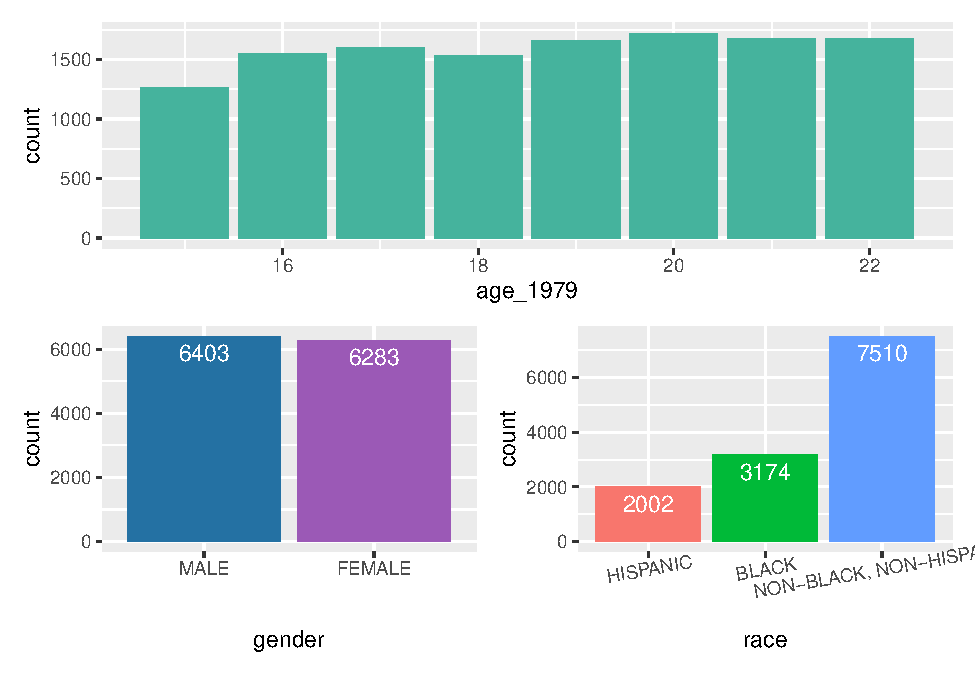
\includegraphics{report_files/figure-latex/valid-age-1.pdf}
\caption{Subjects' Age Distribution}
\end{figure}

\hypertarget{robust-linear-model-for-influential-values-treatment}{%
\subsubsection{Robust Linear Model for Influential Values
Treatment}\label{robust-linear-model-for-influential-values-treatment}}

\hypertarget{summary}{%
\section*{Summary}\label{summary}}
\addcontentsline{toc}{section}{Summary}

\hypertarget{refs}{}
\leavevmode\hypertarget{ref-Chatfield1985TIEo}{}%
Chatfield, C. 1985. ``The Initial Examination of Data.'' \emph{Journal
of the Royal Statistical Society. Series A. General} 148 (3): 214--53.

\leavevmode\hypertarget{ref-HuebnerMariannePhD2016Asat}{}%
Huebner, PhD, Marianne, Dr rer. nat Vach Werner, and PhD le Cessie
Saskia. 2016. ``A Systematic Approach to Initial Data Analysis Is Good
Research Practice.'' \emph{The Journal of Thoracic and Cardiovascular
Surgery} 151 (1): 25--27.

\leavevmode\hypertarget{ref-brolgar}{}%
Tierney, Nicholas, Di Cook, and Tania Prvan. 2020. \emph{Brolgar: BRowse
over Longitudinal Data Graphically and Analytically in R}.
\url{https://github.com/njtierney/brolgar}.

\leavevmode\hypertarget{ref-ggplot2}{}%
Wickham, Hadley. 2016. \emph{Ggplot2: Elegant Graphics for Data
Analysis}. Springer-Verlag New York.
\url{https://ggplot2.tidyverse.org}.

\leavevmode\hypertarget{ref-stringr}{}%
---------. 2019. \emph{Stringr: Simple, Consistent Wrappers for Common
String Operations}. \url{https://CRAN.R-project.org/package=stringr}.

\leavevmode\hypertarget{ref-tidyr}{}%
---------. 2020. \emph{Tidyr: Tidy Messy Data}.
\url{https://CRAN.R-project.org/package=tidyr}.

\leavevmode\hypertarget{ref-dplyr}{}%
Wickham, Hadley, Romain François, Lionel Henry, and Kirill Müller. 2020.
\emph{Dplyr: A Grammar of Data Manipulation}.
\url{https://CRAN.R-project.org/package=dplyr}.

\bibliographystyle{unsrt}
\bibliography{references.bib}


\end{document}
